\documentclass{article}

\thispagestyle{empty}

%\documentclass{minimal}
\usepackage[a4paper,margin=0.5 cm]{geometry}

\usepackage{tikz}
\usepackage{graphicx}

\usetikzlibrary{positioning,shapes,shadows,arrows, shapes.symbols,shapes.geometric}

\usepackage{ragged2e}
\usepackage[T1]{fontenc}
\usepackage[utf8]{inputenc}
\usepackage{textcomp}
\usepackage{eurosym}

\begin{document}
 
\tikzstyle{rect_round} = [rectangle, draw=black, rounded corners, fill=white!40, drop shadow, anchor=north, text=black, text width= 5cm, minimum height = 3 cm,  minimum width = 5 cm]


\tikzset{
  multidocument/.style={
    shape=tape,
    draw,
    fill=white,
    tape bend top=none,
    double copy shadow}}
    
\tikzstyle{multidoc} = [multidocument, draw=black, rounded corners, fill=white!40, drop shadow, anchor=north, text=black, text width= 5cm, minimum height = 3 cm,  minimum width = 5 cm]
    


\begin{figure} [ht]
\begin{center}
\begin{tikzpicture}[node distance=3.5cm, auto]


\node (step1) [rect_round, rectangle split, rectangle split parts=2, text width= 6.2cm,]
        {
            \textbf{Technical specifications}  
            \nodepart{second} $\bullet$ Type of the structure (bridge, wind turbine, etc.) \\ $\bullet$ Type of material (steel, concrete, composite)\\
            $\bullet$ Component details\\ 
            $\bullet$ $\cdots$ 
        };
 

        
\node (step2) [rect_round, rectangle split, rectangle split parts=2, below of = step1, node distance=3.5cm, text width= 5.2cm,]
        {
            \textbf{Identifying the failure modes} 
            \nodepart{second} $\bullet$ Steel (Fatigue and Corrosion) \\ $\bullet$ Concrete (Carbonation and choloride penetration) \\ 
            $\bullet$ $\cdots$ 
        };

 
\node (step3) [rect_round, rectangle split, rectangle split parts=2, text width= 4.2cm, node distance=6cm, right of= step2]
        {
            \textbf{SHM Information from} 
            \nodepart{second} $\bullet$ Strain gauges \\ $\bullet$ Accelerometers \\ $\bullet$ Extensometers \\ $\bullet$ $\cdots$
        }; 
 
        
\node (step4) [rect_round, rectangle split, rectangle split parts=2, text width= 6cm, below of = step2, node distance=4.4cm]
        {
            \textbf{Updating parameters using SHM} 
            \nodepart{second} $\bullet$ Loading parameters \\ $\bullet$  Stress intensity factor\\ $\bullet$ Carbonation and corrosion rates \\ $\bullet$ $\cdots$ 
        };
        
\node (step5) [rect_round, rectangle split, rectangle split parts=2, text width= 6cm, node distance=2.8cm, below of= step4]
        {
            \textbf{Evaluating performance indicators} 
            \nodepart{second}  
            $\bullet$ Annual reliability index\\
            $\bullet$ Annual risk Index\\
            $\bullet$ $\cdots$ 
            
        };
        
\node (step6) [rect_round, rectangle split, rectangle split parts=2, text width= 7cm, node distance=4.1cm, below of= step5]
        {
            \textbf{Deterioration prediction} 
            \nodepart{second}  
            \begin{center} \includegraphics[width=1\linewidth]{deter.pdf} \end{center}

            
        };        
 
\node (step7) [rect_round, rectangle split, rectangle split parts=2, text width= 4cm, node distance=7cm, left of= step6]
        {
            \textbf{Maintenance effect} 
            \nodepart{second}  
            \begin{center} \includegraphics[width=0.8\linewidth]{effect.pdf} \end{center}           
        };  
        
\node (step8) [rect_round, rectangle split, rectangle split parts=2, text width= 4.5cm, node distance=3.7cm, below of= step7]
        {
            \textbf{Maintenance cost} 
            \nodepart{second}  
            $\bullet$ Associated costs to maintenance and repair actions?\\
            $\bullet$ Associated cost to inspections and monitoring actions?\\
            $\bullet$ $\cdots$
            
        };        
\node (step9) [rect_round, rectangle split, rectangle split parts=2, text width= 9cm, node distance=6.8cm, below of= step6]
        {
            \textbf{Optimazation of maintenance planning} 
            \nodepart{second}  
            $\bullet$ Optimum expected extended service life\\
            $\bullet$ Optimum maintenance and inspection strategy\\
            $\bullet$ Optimum excpected cost of service life\\
            $\bullet$ $\cdots$ 
            
        };            

\draw [-stealth, thick, line width=0.7mm] (step1) -- (step2);
\draw [-stealth, thick, line width=0.6mm] (step3) -- ++ (-3,0) -- ++(0,-2.5) -- ++(-1.5,0) -- (step4);
%\draw [-stealth, thick, line width=0.6mm] (step3) --++ (-4.5,0)--++ (step4);      
\draw [-stealth, thick, line width=0.7mm] (step2) -- (step4);
\draw [-stealth, thick, line width=0.7mm] (step4) -- (step5);
\draw [-stealth, thick, line width=0.7mm] (step5) -- (step6);
\draw [-stealth, thick, line width=0.7mm] (step6) -- (step9);
\draw [-stealth, thick, line width=0.6mm] (step7) -- ++(3.2,0) -- ++(0,-3.5) -- ++(3,0) -- (step9);
\draw [-stealth, thick, line width=0.6mm] (step8) -- ++(3,0) -- ++(0,-0.75) -- ++(3,0) --  (step9);
\end{tikzpicture}
\end{center}
\end{figure}
\end{document}
